%%%%%%%%%%%%%%%%%%%%%%%%%%%%%%%%%%%%%%%%%%%%%%%%%%%%%%%%%%%%%%%%%%%%%%%%%%%%%%%%
%%            _   _            __   ____                                      %%
%%           / / | |          / _| |  __|                                     %%
%%           | |_| |  _   _  / /   | |_                                       %%
%%           |  _  | | | | | | |   |  _|                                      %%
%%           | | | | | |_| | \ \_  | |__                                      %%
%%           |_| |_| \_____|  \__| |____| microLab                            %%
%%                                                                            %%
%%           Bern University of Applied Sciences (BFH)                        %%
%%           Quellgasse 21                                                    %%
%%           Room HG 4.33                                                     %%
%%           2501 Biel/Bienne                                                 %%
%%           Switzerland                                                      %%
%%                                                                            %%
%%           http://www.microlab.ch                                           %%
%%%%%%%%%%%%%%%%%%%%%%%%%%%%%%%%%%%%%%%%%%%%%%%%%%%%%%%%%%%%%%%%%%%%%%%%%%%%%%%%
%% GECKO4com
\documentclass [10pt,a5paper,twoside,openright]{book}
\usepackage{times}
\usepackage{amsmath}
\usepackage{amsfonts}
\usepackage {graphicx}
\usepackage{changepage}
\usepackage{geometry}
\usepackage{fancyhdr}
\usepackage{array}
\usepackage{calc}
\usepackage{chapterbib}
\renewcommand{\bibname}{References}
\usepackage{subfigure}
\usepackage{multirow}
\usepackage{pifont}
\usepackage[small,bf,nooneline]{caption}
\usepackage[printonlyused,withpage]{acronym}
\usepackage[sty]{fncychap}
\graphicspath{{figs/}}
\pagestyle{fancy}
\geometry{a5paper,hdivide={1cm,,1cm},vdivide={1.5cm,,1.5cm},includeall,
          marginparwidth=1.2cm,marginparsep=0.3cm,bindingoffset=1cm,
          heightrounded,headheight=1cm,reversemp,asymmetric}
\renewcommand{\headrulewidth}{0pt}
\fancyhfoffset[LO,LE]{\marginparwidth+\marginparsep}
\setlength{\headwidth}{\textwidth}
\addtolength{\headwidth}{\marginparwidth}
\addtolength{\headwidth}{\marginparsep}
\fancyhf{}
\fancypagestyle{plain}{}
\renewcommand{\chaptermark}[1]{\markboth{#1}{}}
\renewcommand{\sectionmark}[1]{\markright{#1}{}}

\newlength{\skipleft}
\setlength{\skipleft}{\marginparwidth}
\addtolength{\skipleft}{\marginparsep}

\makeatletter
\def\cleardoublepage{\clearpage\if@twoside \ifodd\c@page\else
   \hbox{}
   \thispagestyle{empty}
   \newpage
   \if@twocolumn\hbox{}\newpage\fi\fi\fi}
\def\@seccntformat#1{\protect\makebox[0pt][r]{\csname the#1\endcsname\quad}}
\ChNumVar{\fontsize{76}{80}\usefont{OT1}{pzc}{m}{n}\selectfont}
\ChTitleVar{\Large\sffamily\bfseries}
\renewcommand{\DOCH}{\vskip -80pt}
\renewcommand{\DOTI}[1]{%
   \hskip -\skipleft
   \begin{tabular*}{\headwidth}{m{1.7cm}m{\textwidth}}
            \CNoV\thechapter
            &
            \CTV\FmTi{#1}
            \\
            \hline
   \end{tabular*}
            \vskip 20 pt}
\renewcommand{\DOTIS}[1]{
   \vskip -80 pt
   \centering\CTV\FmTi{#1}
   \vskip -30 pt}
\makeatother
\sectionbib{\section*}{section}
\newcommand{\notocsection}[1]{%
    \refstepcounter{section}%
    \section*{\thesection \quad #1}}%
%------------------------------------------------------------------------------
% navi and reading infos
\usepackage{marvosym}
\newcommand{\note}{\marginpar{\LARGE\Info}}
\newcommand{\important}{\marginpar{\LARGE\Pointinghand}}
%
\author {Dr. T.J.H. Kluter}
\title {GECKO4com\\Technical Reference Manual}
%
\begin {document}
%%%%%%%%%%%%%%%%%%%%%%%%%%%%%%%%%%%%%%%%%%%%%%%%%%%%%%%%%%%%%%%%%%%%%%%%%%%%%%%%
%%            _   _            __   ____                                      %%
%%           / / | |          / _| |  __|                                     %%
%%           | |_| |  _   _  / /   | |_                                       %%
%%           |  _  | | | | | | |   |  _|                                      %%
%%           | | | | | |_| | \ \_  | |__                                      %%
%%           |_| |_| \_____|  \__| |____| microLab                            %%
%%                                                                            %%
%%           Bern University of Applied Sciences (BFH)                        %%
%%           Quellgasse 21                                                    %%
%%           Room HG 4.33                                                     %%
%%           2501 Biel/Bienne                                                 %%
%%           Switzerland                                                      %%
%%                                                                            %%
%%           http://www.microlab.ch                                           %%
%%%%%%%%%%%%%%%%%%%%%%%%%%%%%%%%%%%%%%%%%%%%%%%%%%%%%%%%%%%%%%%%%%%%%%%%%%%%%%%%
\begin{adjustwidth}{-\skipleft}{0pt}
\begin{center}
\huge{{\sc GECKO4com}}\\
\large{Technical Reference Manual}\\
\large{Revision 1.0.1}\\
Dr. Theo Kluter
\end{center}
\vspace*{2cm}%
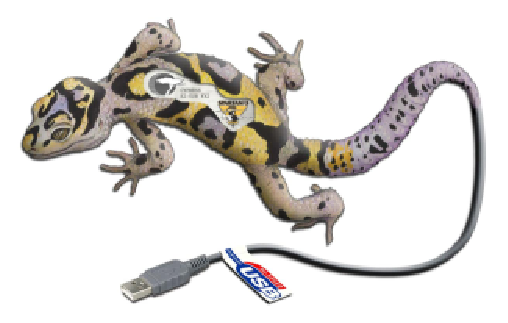
\includegraphics[width=\columnwidth]{figs/gecko3logo}%
\vspace*{2cm}\\%
{\sc GECKO} is an active project at HuCE-microLab where various team members
have made their contributions. Currently the following researchers are
involved:\\
Andreas~Habegger, %
Benjamin~Habegger, %
Fabian~Nenniger, %
Dr.~Theo~Kluter, \\
Prof.~Dr.~Josef~Goette, %
Prof.~Dr.~Marcel~Jacomet.\\
 \\

\includegraphics[height=0.5cm]{figs/HuCEmicrolab-nofont}\hspace*{4.5cm}%
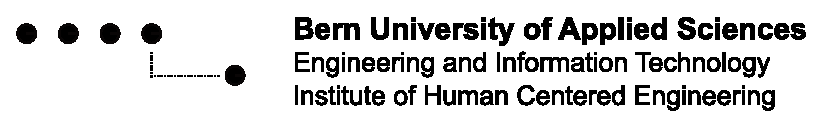
\includegraphics[height=0.5cm]{figs/BFHhuceENnofonts}\\
\end{adjustwidth}

%\maketitle
%
%-----------------------------------------------------------------------------
%
\begin{adjustwidth}{-\skipleft}{0pt}
   \frontmatter
   \tableofcontents
\end{adjustwidth}
%
%-----------------------------------------------------------------------------
%
\mainmatter
\fancyhead[LE]{\textsl{\leftmark}}
\fancyhead[RE]{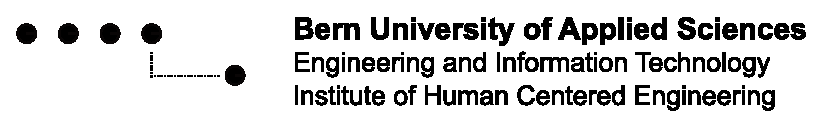
\includegraphics[height=0.5cm]{figs/BFHhuceENnofonts}}
\fancyhead[LO]{
\includegraphics[height=0.5cm]{figs/HuCEmicrolab-nofont}}
\fancyhead[RO]{\textsl{\rightmark}}
\fancyfoot[LE,RO]{\thepage}
\renewcommand{\headrulewidth}{0.4pt}
%
%-----------------------------------------------------------------------------
%
\include{intro_symbols}
%
%-----------------------------------------------------------------------------
%
%%%%%%%%%%%%%%%%%%%%%%%%%%%%%%%%%%%%%%%%%%%%%%%%%%%%%%%%%%%%%%%%%%%%%%%%%%%%%%%%
%%            _   _            __   ____                                      %%
%%           / / | |          / _| |  __|                                     %%
%%           | |_| |  _   _  / /   | |_                                       %%
%%           |  _  | | | | | | |   |  _|                                      %%
%%           | | | | | |_| | \ \_  | |__                                      %%
%%           |_| |_| \_____|  \__| |____| microLab                            %%
%%                                                                            %%
%%           Bern University of Applied Sciences (BFH)                        %%
%%           Quellgasse 21                                                    %%
%%           Room HG 4.33                                                     %%
%%           2501 Biel/Bienne                                                 %%
%%           Switzerland                                                      %%
%%                                                                            %%
%%           http://www.microlab.ch                                           %%
%%%%%%%%%%%%%%%%%%%%%%%%%%%%%%%%%%%%%%%%%%%%%%%%%%%%%%%%%%%%%%%%%%%%%%%%%%%%%%%%
\chapter{Implemented Commands}
\label{chap:commands}
The {\sc GECKO4com} implements 36 {\sc SCPI} commands as shown in
Table~\ref{tab:scpi commands}. The commands starting with a \verb+*+ are
compliant with the IEEE488.1~\cite{ieee488_1} and IEEE488.2~\cite{ieee488_2}
standards and will not be described in this chapter. The exception to the above
is the description of the \verb+*PUD+, \verb+*PUD?+ and \verb+*RST+ commands.
\begin{table}[hb]
\begin{tabular}{|l|l|l|l|}
\hline
\verb+*CLS+&\verb+*ESE+&\verb+*ESE?+&\verb+*ESR?+\\
\hline
\verb+*IDN?+&\verb+*IST?+&\verb+*OPC+&\verb+*OPC?+\\
\hline
\verb+*PUD+&\verb+*PUD?+&\verb+*RST+&\verb+*SRE+\\
\hline
\verb+*SRE?+&\verb+*STB?+&\verb+*TST?+&\verb+*WAI+\\
\hline
\verb+BITFLASH+&\verb+BITFLASH?+&\verb+BOARD?+&\verb+CONFIG+\\
\hline
\verb+ERASE+&\verb+FIFO+&\verb+FIFO?+&\verb+FPGA+\\
\hline
\verb+FPGA?+&\verb+HEXSWITCH+&\verb+HEXSWITCH?+&\verb+IDENTIFY+\\
\hline
\verb+TRANS+&\verb+USERRESET+&\verb+VGA:BGCOL+&\verb+VGA:CLEAR+\\
\hline
\verb+VGA:CURSOR+&\verb+VGA:CURSOR?+&\verb+VGA:FGCOL+&\verb+VGA:PUTSTR+\\
\hline
\end{tabular}
\caption{{\sc SCPI} commands implemented in the {\sc GECKO4com}}
\label{tab:scpi commands}
\end{table}
%-----------------------------------------------------------------------------
\section{Protected User Data}
\label{sec: PUD}
The IEEE488.1~\cite{ieee488_1} and IEEE488.2~\cite{ieee488_2} standards describe
the \verb+*PUD+ and \verb+*PUD?+ as optional commands. These two commands
provide a Protected User Data (PUD) area of at least 63 bytes. The {\sc GECKO4com}
implements a PUD of 2048 bytes and violates the standard in the protection
requirement.\\
 \\
\textbf{Reading the PUD area:}\\
When executing the \verb+*PUD?+ command the {\sc GECKO4com} puts the contents of
the complete PUD memory (2048 bytes) in the output queue. The PUD memory can
only be read completely; there exist no possibility to read only a part of it.\\
 \\
\textbf{Writing the PUD area:}\\
The PUD area can be written with the \verb*+*PUD <payload>+ command. The number
of spaces (\verb*+ +) between the command and the payload must be exactly
one. All the other spaces are interpreted as payload. The size of
the payload can be anywhere between 1 and 2048 bytes. Upon receiving this
command the {\sc GECKO4com} will start writing at address 0 of the PUD memory.
If the payload size is more than 2048 bytes the {\sc GECKO4com} will wrap around
and overwrite earlier written data. After having received the payload, the {\sc
GECKO4com} will store the complete 2048 bytes of the PUD memory in an external
attached flash.\\
\textit{Note:  If there is no Flash chip mounted on the {\sc GECKO4main}, the
PUD memory area will become volatile.\note}\\
\textit{Important: Each execution of the} \verb+*PUD+ \textit{command will initiate a
sector erase/program cycle of the attached Flash chip; therefore, the number of 
the} \verb+*PUD+ \textit{command invocation is limited by the number of 
sector erase cycles specified by the Flash chip manufacturer.\important}\\
 \\
\textbf{PUD memory organization:}\\
The PUD memory organization is shown in Figure~\ref{fig:PUD mem org}.
\begin{figure}
\centering%
\includegraphics[width=0.7\columnwidth]{figs/pud_memory_org}
\caption{Memory organization of the PUD area. The memory is continues; the
64-byte blocks are only shown to indicate the thirteen ASCII lines.}
\label{fig:PUD mem org}
\end{figure}
The area between \verb+0x000+ and \verb+0x4BF+ is completely user definable;
however the area between \verb+0x4C0+ and \verb+0x7FF+ is used to store thirteen
lines of sixty four ASCII characters that are displayed in the Static User Window
 (SUW) of the VGA-controller (see Chapter~\ref{sec: vga}).\\
  \\
\textbf{PUD command error handling:}\\
Both the \verb+*PUD+ and \verb+*PUD?+ are always executed successfully; therefore
there is no command error generated for either of these commands.
%-----------------------------------------------------------------------------
\section{Global Reset}
The {\sc GECKO4com} provides the means to activate the Global Reset. It is
important to not confuse the Global Reset with the User Reset as described in
Chapter~\ref{chap:user_reset}. The {\sc GECKO4com} activates the Global Reset by
pulling the signal actively low. In case of a deactivated Global Reset, the
{\sc GECKO4com} leaves this pin floating. No pull-up on this signal is provided
by the {\sc GECKO4com}. For more details on the requirements of the Global Reset
(GR) signal please refer to the {\sc GECKO4main} technical reference
guide~\cite{gecko4main}.\\
 \\
\textbf{GR activation:}\\
There are two situations for which the {\sc GECKO4com} activates the Global
Reset line, namely:
\begin{enumerate}
\item \textbf{Unconfigured FPGA:} If the user FPGA on the {\sc GECKO4main} is
not configured the Global Reset line is kept activate.
In case no user FPGA is mounted, the the Global Reset line is deactivated.
\item \textbf{Reset command:} By executing the \verb+*RST+ command, the Global
Reset line is activated for a period between 10~ms and 11~ms.
\end{enumerate}
\textit{Important: The {\sc GECKO4com} is uneffected by the state of the Global Reset
line.\important}\\
 \\
\textbf{GR command error handling:}\\
The \verb+*RST+ command always executes correctly; therefore there is no command
error generated for this command.
%-----------------------------------------------------------------------------
\section{User Reset}
\label{chap:user_reset}
Contrary to the Global Reset signal the User Reset signal is only connected to
the user FPGA on the {\sc GECKO4main}. This User Reset signal provides the means
of resetting the logic inside the user FPGA without effecting attached
boards. The User Reset (UR) signal is an \emph{active low} signal that is actively
driven for both a \verb+1+ and a \verb+0+. The User Reset signal is connected to
pin \textbf{Y9} of the user FPGA.\\
 \\
\textbf{UR activation:}\\
There are two situations for which the User Reset line is activated, namely:
\begin{enumerate}
\item \textbf{Unconfigured FPGA:} If the user FPGA on the {\sc GECKO4main} is
not configured the User Reset line is kept activate up to a period of 10~ms to
11~ms after the done line of the user FPGA went high.
In case no user FPGA is mounted, the User Reset line is deactivated.
\item \textbf{Reset command:} By executing the \verb+USERRESET+ command, the
User Reset line is activated for a period between 10~ms and 11~ms.
\end{enumerate}
\textit{Important: The {\sc GECKO4com} is uneffected by the state of the User Reset
line.\important}\\
\textit{Important: The User Reset line is uneffected by the state of the Global
Reset line.\important}\\
 \\
\textbf{UR command error handling:}\\
The \verb+USERRESET+ command always executes correctly; therefore there is no command
error generated for this command.
%-----------------------------------------------------------------------------
\section{Bitfile Storage}
To be able to operate the {\sc GECKO4main} in an environment where a USB
connection is not wanted, the {\sc GECKO4com} provides the means to store the
user FPGAs configuration in a non-volatile memory. The user FPGAs configuration,
further referred to as \emph{bitfile}, is generated by the Xilinx toolchain and
consists of a variable length header and the configuration data in form of a
bitstream~\cite{FPGAFAQ_0026}. The {\sc GECKO4com} provides four commands to
manipulate the bitfile storage.
\begin{itemize}
\item \verb*+BITFLASH <bitfile>+. This command stores the \verb+<bitfile>+ in
the non-volatile memory of the {\sc GECKO4com}. This command can take upto two
seconds to complete due to the speed of the non-volatile memory. This command
is only succesfull in case of an empty non-volatile memory, otherwise an
execution error is generated.\\
\textit{Important: (1) The {\sc GECKO4com} does not control if the provided
bitfile is suitable for the mounted user FPGA and
(2) only a single space (}\verb*+ +\textit{)  must be provided between the command and
the bitfile.}
\item \verb+CONFIG+. This command configures the user FPGA with the bitfile
stored in the non-volatile memory. If the non-volatile memory does not contain a
bitfile an execution error is generated.
\item \verb+ERASE+. This command erases the non-volatile memory and must be
provided before the programming of a new bitfile into the non-volatile memory.
This command can take several seconds to complete.
\item \verb+BITFLASH?+. This command returns \verb+EMPTY+ if the non-volatile
memory is empty, and the stored bitfile otherwise.
\end{itemize}
\textit{Note: It is highly discouraged to use the }\verb+BITFLASH <bitfile>+
\textit{ and }
\verb+ERASE+ \textit{ commands in a script due to their execution time. Most likely a
time-out error is generated on the USBTMC protocol due to these execution
times. \note}
%-----------------------------------------------------------------------------
\section{{\sc GECKO4main} information}
\label{sec: main info}
The {\sc GECKO4com} provides two commands to report the current status of the
{\sc GECKO4main} system. Both these commands always execute successfully and
return an ASCII string.
\begin{itemize}
\item \verb+FPGA?+. This command returns the detected user FPGA type and its
configuration state. Possible user FPGAs are listed in the {\sc GECKO4main}
Technical Reference Manual~\cite{gecko4main}. If no user FPGA is
mounted or the {\sc GECKO4com} was unable to determine the FPGA type this
command returns the message \emph{No FPGA mounted or unknown FPGA type} and all
user FPGA manipulations are prohibited.
\item \verb+BOARD?+. This command returns the powering status, e.g. USB
supplied, GENIO1 supplied, powering BUS, of the {\sc GECKO4main} and the status
of the {\sc GECKO4com}'s non-volatile memory (empty or programmed) [see previous
section].
\end{itemize}
Furthermore the {\sc GECKO4com} provides the means of identifying optically an
attached {\sc GECKO4main} by means of the command \verb+IDENTIFY+. After
execution of this command the eight LEDs of {\sc GECKO4main} will start to
become red, afterwards they change to green and finally they will go off one
after the other. This sequence lasts for approximately one second.
%-----------------------------------------------------------------------------
\section{User FPGA configuration}
The {\sc GECKO4com} provides the means to configure the user FPGA. This
configuration is independent of the current state of the user FPGA. This means
that the user FPGA can be configured as many times as required and with as many
bitfiles as wanted. By this flexibility of the {\sc GECKO4com} progression
testing and scripted simulations/emulations. The configuration time for even the
largest Spartan 3 5000 FPGA is only a few tens of milliseconds.

The command to configure the user FPGA is \verb*+FPGA <bitfile>+. This command
\textbf{must} only contain one space (\verb*+ +). In case no user FPGA is
mounted or the {\sc GECKO4com} was unable to detect the mounted user FPGA  this
command will generate an execution error.\\
\textit{Important: The {\sc GECKO4com} does not control if the provided bitfile
is suitable for the mounted user FPGA. It is up to the user to make sure that
the bitfile that is uploaded is generated for the correct user FPGA type. In
case a wrong bitfile is uploaded the command will execute successfully; however
the user FPGA will refuse to load it. To be able to see if the user FPGA has
been configured correctly the }\verb+FPGA?+\textit{ command can be used to ask
the current status if the user FPGA. \important}
%-----------------------------------------------------------------------------
\section{Mechanical Switch}
\label{sec: hexswitch}
The {\sc GECKO4main} provides a hexadecimal encoded switch that is further
referred to as \emph{hexswitch}. The {\sc GECKO4com} provides two commands to
manipulate this switch.
\begin{itemize}
\item \verb*+HEXSWITCH <value>+. This command overrides the mechanical switch and
forces the \verb+<value>+ to appear on both the user FPGA side (see
Chapter~\ref{sec:mem map}) as well as from the PC side. The parameter
\verb+<value>+ can be any of the set [0-9,A-F,a-f]. Between the command and the
parameter \verb+<value>+ there may be as many spaces (\verb*+ +) as wanted. This
command executes successfully as long as the parameter \verb+<value>+ is in the
set mentioned before. This command is persistent until either the board is
powered, or an \verb+INITIATE_CLEAR+ USBTMC message~\cite{usbtmc} is send. This
command may be send as often as required and will each time override the
previous value send.
\item \verb+HEXSWITCH?+. This command reports the current state of the hexswitch
or the override value if a \verb+HEXSWITCH+ command has been issued before this
command. The result of this command is an ASCII character of the set [0-9,A-F]
followed by a new-line character (\verb+0x0A+).
\end{itemize}
%-----------------------------------------------------------------------------
\section{User FPGA communication}
The {\sc GECKO4com} provides three commands that allows for communication
between the PC and the user FPGA. These commands are \verb+FIFO+, \verb+FIFO?+,
and \verb+TRANS+. More information on these commands and the protocols involved
can be found in Chapter~\ref{chap:fpga}.
%-----------------------------------------------------------------------------
\section{VGA controller}
\label{sec: vga commands}
The {\sc GECKO4com} provides a VGA controller not only for debug purposes but
also for demonstration purposes. The VGA controller implemented in the {\sc
GECKO4com} has one USBTMC window (see Chapter~\ref{sec: vga} for further
information). The commands to manipulate this window are listed below.
\begin{itemize}
\item \verb*+VGA:FGCOL <value>+. This command sets the forground color of the
VGA window. The parameter \verb+<value>+ can be any character between \verb+0+
and \verb+7+ (see also Chapter~\ref{sec: vga}).
\item \verb*+VGA:BGCOL <value>+. This command sets the background color of the
VGA window. The parameter \verb+<value>+ can be any character between \verb+0+
and \verb+7+ (see also Chapter~\ref{sec: vga}).
\item \verb+VGA:CLEAR+. This command clears the VGA window and puts the cursor
on the left top position of the screen.
\item \verb+VGA:CURSOR?+. This command returns the current cursor position. The
format returned is a string in the form \verb+<x>,<y>+ where
$\text{x}\in[0..63]$ and $\text{y}\in[0..31]$.
\item \verb*+VGA:CURSOR <x>,<y>+. This command sets the current cursor position
to (x,y). The parameters: $\text{x}\in[0..63]$ and $\text{y}\in[0..31]$.\\
\textit{Note: The parameters x and y must be specified as ASCII characters and
not as bytes, e.g. 31 equals the character ``3'' (0x33) followed by the
character ``1'' (0x31).\note}
\item \verb*+VGA:PUTSTR <string>+. This command displays all the bytes following
the space (\verb*+ +) at the current cursor position on the VGA window as ASCII
characters. A new-line character (\verb+0x0A+) will forse a new line and all
bytes with a value smaller than the ASCII character space (\verb+0x20+) will be
ignored.\\
\textit{Important: No commands can be concatinated with this command. Doing so
will ``print'' them on the VGA screen rather than executing them.\important}
\end{itemize}
%-----------------------------------------------------------------------------
\section{The Status Byte Register}
\label{sec: SBR}
The IEEE488.1~\cite{ieee488_1} and IEEE488.2~\cite{ieee488_2} standards define
an obligatory status byte register as shown in Figure~11-8 in the
IEEE488.2~\cite{ieee488_2} standard. The {\sc GECKO4com} implements this
register with the obligatory \emph{MSS}, \emph{ESB}, and \emph{MAV} bits.
Besides from these obligatory bits, the {\sc GECKO4com} implements 2 extra
status bits.
\begin{itemize}
\item \textbf{Bit 3.} Bit 3 in the Status Byte Register indicates when \verb+1+
that the user FPGA is configured and running. When this bit is \verb+0+ the user
FPGA is either not present or not configured.
\item \textbf{Bit 2.} Bit 2 in the Status Byte Register indicates when \verb+1+
that the {\sc GECKO4com} is in \emph{transparent mode} (see Chapter~\ref{sec:trans mode}).
When this bit is \verb+0+ the {\sc GECKO4com} is in normal operation mode.
\end{itemize}
If the {\sc GECKO4com} is in \emph{transparent mode} it does only supply the
\emph{MSS} bit, the \emph{MAV} bit, and the transparent bit (bit 2) of the
Status Byte Register. It is left to the user FPGA to provide the following bits:
\begin{itemize}
\item \textbf{Bit 7 (ESB).} In \emph{transparent mode} the user FPGA {\sc must}
provide the \emph{ESB} bit. This bit is at pin \verb+AE6+ of the user FPGA and
of type {\sc lvcmos25}.
\item \textbf{Bit 3.} In \emph{transparent mode} this bit is user definable by
the user FPGA. This bit is at pin \verb+AE8+ of the user FPGA and of type {\sc
lvcmos25}.
\end{itemize}
For the user FPGA to know if the {\sc GECKO4com} is in \emph{transparent mode},
the pin \verb+AD6+ at the user FPGA is a copy of bit 2 in the Status Byte
Register. Figure~\ref{fig:stb} shows the Status Byte Register as provided by the
{\sc GECKO4com}.
\begin{figure}[t]
\centering%
\includegraphics[width=0.8\columnwidth]{figs/status_byte_register}
\caption{The Status Byte Register as defined by the {\sc GECKO4com}.}
\label{fig:stb}
\end{figure}
%-----------------------------------------------------------------------------
\def\srt#1{}
\begin{thebibliography}{10}
\bibitem{FPGAFAQ_0026}
Alan Nishioka and Philip Freidin,
\newblock{\em FPGA-FAQ 0026---{T}ell me about the .{BIT} file format.}
\newblock \verb+www.fpga-faq.com+, Nov. 2001

\bibitem{gecko4main}
Dr. Theo Kluter,
\newblock{\em {\sc GECKO4main} {T}echnical {R}eference {M}anual.}
\newblock Bern University of Applied Sciences, Biel/Bienne, Switzerland, 2011.

\bibitem{ieee488_1}
IEEE, Inc.
\newblock{\em {IEEE} {S}tandard {C}odes, {F}ormats, {P}rotocols, and
{C}ommon {C}ommands for {U}se {W}ith {IEEE} {S}td 488.1-1987, {IEEE}
{S}tandard {D}igital {I}nterface for {P}rogrammable {I}nstrumentation.}
\newblock ISBN 1-55937-238-9, New York, 1992.

\bibitem{ieee488_2}
IEC and IEEE.
\newblock{\em {IEC} 60488-2, {IEEE} 488.2: {S}tandard digital interface for
programmable instrumentation --- {P}art 2: {C}odes, formats, protocols and
common commands.}
\newblock First edition, 2005-05.

\bibitem{usbtmc}
USB Implementers Forum, Inc.
\newblock{\em {U}niversal {S}erial {B}us {T}est and {M}easurement {C}lass
{S}pecification ({USBTMC})--{R}evision 1.0.}
\newblock April, 2003
\end{thebibliography}

%
%-----------------------------------------------------------------------------
%
%%%%%%%%%%%%%%%%%%%%%%%%%%%%%%%%%%%%%%%%%%%%%%%%%%%%%%%%%%%%%%%%%%%%%%%%%%%%%%%%
%%            _   _            __   ____                                      %%
%%           / / | |          / _| |  __|                                     %%
%%           | |_| |  _   _  / /   | |_                                       %%
%%           |  _  | | | | | | |   |  _|                                      %%
%%           | | | | | |_| | \ \_  | |__                                      %%
%%           |_| |_| \_____|  \__| |____| microLab                            %%
%%                                                                            %%
%%           Bern University of Applied Sciences (BFH)                        %%
%%           Quellgasse 21                                                    %%
%%           Room HG 4.33                                                     %%
%%           2501 Biel/Bienne                                                 %%
%%           Switzerland                                                      %%
%%                                                                            %%
%%           http://www.microlab.ch                                           %%
%%%%%%%%%%%%%%%%%%%%%%%%%%%%%%%%%%%%%%%%%%%%%%%%%%%%%%%%%%%%%%%%%%%%%%%%%%%%%%%%
\chapter{Bus Interface}
To be able to use the {\sc GECKO4com} from the user FPGA it provides a bus
interface. The provided IP-cores in the {\sc GECKO4com} can be accessed through
this bus and are accessed by a memory map.
%-------------------------------------------------------------------------------
\section{Bus Signals}
Table~\ref{tab:gecko4 bus signals} list all the bus signals as used by the {\sc
GECKO4com}, their direction, and their pin on the user FPGA. The bi-directional
signals (marked by {\sc bidir}) are forced either by the {\sc GECKO4com} or the
user FPGA depending on the bus protocol (see Appendix~\ref{appen:bus} and
Chapter~\ref{sec:bus prot}).
%-------------------------------------------------------------------------------
\begin{table}[hb]
\begin{tabular}{|l|c|c||l|c|c|}
\hline
\textbf{Signal}&\textbf{Type}&\textbf{Pin}&
\textbf{Signal}&\textbf{Type}&\textbf{Pin}\\
\hline
\hline
$\overline{\text{start trans}}$&{\sc uf-gc} {\sc al}&\verb+AB11+&
$\overline{\text{end trans}}$&{\sc bidir} {\sc al}&\verb+W11+\\
\hline
$\overline{\text{valid lo}}$&{\sc bidir} {\sc al}&\verb+AB10+&
$\overline{\text{valid hi}}$&{\sc bidir} {\sc al}&\verb+AC10+\\
\hline
$\overline{\text{error}}$&{\sc gc-uf} {\sc al}&\verb+AA10+&
$\overline{\text{start send}}$&{\sc gc-uf} {\sc al}&\verb+AA11+\\
\hline
request irq&{\sc gc-uf}&\verb+AC11+&
error irq&{\sc gc-uf}&\verb+Y10+\\
\hline
available irq&{\sc gc-uf}&\verb+AF8+&
$\overline{\text{bus reset}}$&{\sc uf-gc} {\sc al}&\verb+Y11+\\
\hline
data cntrl 0&{\sc bidir}&\verb+AD4+&
data cntrl 1&{\sc bidir}&\verb+AD5+\\
\hline
data cntrl 2&{\sc bidir}&\verb+AE4+&
data cntrl 3&{\sc bidir}&\verb+AE5+\\
\hline
data cntrl 4&{\sc bidir}&\verb+AF4+&
data cntrl 5&{\sc bidir}&\verb+AF5+\\
\hline
data cntrl 6&{\sc bidir}&\verb+W12+&
data cntrl 7&{\sc bidir}&\verb+W13+\\
\hline
data cntrl 8&{\sc bidir}&\verb+Y12+&
data cntrl 9&{\sc bidir}&\verb+Y13+\\
\hline
data cntrl 10&{\sc bidir}&\verb+AA13+&
data cntrl 11&{\sc bidir}&\verb+AD12+\\
\hline
data cntrl 12&{\sc bidir}&\verb+AA6+&
data cntrl 13&{\sc bidir}&\verb+AA7+\\
\hline
data cntrl 14&{\sc bidir}&\verb+AB6+&
data cntrl 15&{\sc bidir}&\verb+AB7+\\
\hline
bus clock&{\sc gc-uf}&\verb+AE13+&
\multicolumn{3}{c|}{\emph{All signals:} {\sc lvcmos25}}\\
\hline
\end{tabular}
\caption{The signals of the bus provided by the {\sc GECKO4com}. {\sc al}
represents active low. {\sc uf-gc} represents a signal driven by the user FPGA
and consumed by the {\sc GECKO4com}. {\sc gc-uf} represents a signal driven by
the {\sc GECKO4com} and consumed by user FPGA. {\sc bidir} represents a
bi-directional signal.}
\label{tab:gecko4 bus signals}
\end{table}
%-------------------------------------------------------------------------------
The signals
marked with {\sc al} are active low signals. The signals marked with {\sc gc-uf}
are driven by (outputs of) the {\sc GECKO4com}. The signals marked with {\sc
uf-gc} are driven by (outputs of) the user FPGA.
The bus is synchrone and is clocked with the 48MHz clock available on pin
\verb+AE13+.
%-------------------------------------------------------------------------------
\section{Memory Map}
\label{sec:mem map}
The IP cores of the {\sc GECKO4com} are available by the memory map shown in
Table~\ref{tab:gecko4 memory map}.
%-------------------------------------------------------------------------------
\begin{table}[hp]
\begin{tabular}{|c|l|c|}
\hline
\textbf{Address}&\textbf{Function}&\textbf{Access}\\
\hline
\hline
\verb+0x00+&Tx-fifo data write&{\sc wo} {\sc burst}\\
\hline
\verb+0x01+&Tx-fifo package size write&{\sc wo} {\sc burst}\\
\hline
\verb+0x02+&Nr. of bytes in TX-fifo&{\sc ro} {\sc burst}\\
\hline
\verb+0x03+&Max. size in bytes of TX-fifo&{\sc ro} {\sc burst}\\
\hline
\verb+0x04+&Nr. of shorts in TX-fifo&{\sc ro} {\sc burst}\\
\hline
\verb+0x05+&Max. size in shorts of TX-fifo&{\sc ro} {\sc burst}\\
\hline
\verb+0x06+&Nr. of words in TX-fifo&{\sc ro} {\sc burst}\\
\hline
\verb+0x07+&Max. size in words of TX-fifo&{\sc ro} {\sc burst}\\
\hline
\verb+0x08+&RX-fifo read data&{\sc ro} {\sc burst}\\
\hline
\verb+0x09+&RX-fifo read data&{\sc ro} {\sc burst}\\
\hline
\verb+0x0A+&Nr. of bytes in RX-fifo&{\sc ro} {\sc burst}\\
\hline
\verb+0x0B+&Max. size in bytes of RX-fifo&{\sc ro} {\sc burst}\\
\hline
\verb+0x0C+&Nr. of shorts in RX-fifo&{\sc ro} {\sc burst}\\
\hline
\verb+0x0D+&Max. size in shorts of RX-fifo&{\sc ro} {\sc burst}\\
\hline
\verb+0x0E+&Nr. of words in RX-fifo&{\sc ro} {\sc burst}\\
\hline
\verb+0x0F+&Max. size in words of RX-fifo&{\sc ro} {\sc burst}\\
\hline
\verb+0x20+&VGA foreground color&{\sc rw}\\
\hline
\verb+0x21+&VGA background color&{\sc rw}\\
\hline
\verb+0x22+&VGA cursor x position&{\sc rw}\\
\hline
\verb+0x23+&VGA cursor y position&{\sc rw}\\
\hline
\verb+0x24+&VGA write ASCII char&{\sc wo}\\
\hline
\verb+0x25+&VGA write dummy to clear screen&{\sc wo}\\
\hline
\verb+0x26+&Buttons status&{\sc ro}\\
\hline
\verb+0x27+&Hex switch status&{\sc ro}\\
\hline
\verb+0x28+&LED 0 mode register&{\sc rw}\\
\hline
\verb+0x29+&LED 1 mode register&{\sc rw}\\
\hline
\verb+0x2A+&LED 2 mode register&{\sc rw}\\
\hline
\verb+0x2B+&LED 3 mode register&{\sc rw}\\
\hline
\verb+0x2C+&LED 4 mode register&{\sc rw}\\
\hline
\verb+0x2D+&LED 5 mode register&{\sc rw}\\
\hline
\verb+0x2E+&LED 6 mode register&{\sc rw}\\
\hline
\verb+0x2F+&LED 7 mode register&{\sc rw}\\
\hline
\end{tabular}
\caption{Memory map of the {\sc GECKO4com} IP cores.}
\label{tab:gecko4 memory map}
\end{table}
%-------------------------------------------------------------------------------
Accessing an address not in
this list will generate a bus error. Furthermore, writing to a read-only
({\sc ro}) or reading from a write-only ({\sc wo}) location will also trigger a bus
error. The addresses marked with {\sc burst} are capable of burst accesses.
Executing a burst on a none burst capable address will trigger a bus error.

The usage of the Tx and Rx fifos (addresses \verb+0x00-0x0F+) are described in
Chapter~\ref{chap:fpga}. The VGA controller (addresses \verb+0x20-0x25+) is described
in Chapter~\ref{sec: vga}. Finally, the buttons, the hexswitch, and the LEDs 
(addresses \verb+0x26-0x2F+) are described in Chapter~\ref{sec:but switch}.
%-------------------------------------------------------------------------------
\section{Bus Protocol}
\label{sec:bus prot}
The implemented bus provides a handshake protocol with a combined
data/address/control path. All signals are related to the positive edge of 48~MHz 
bus clock. The bus clock is generated by the {\sc GECKO4com} and cannot be
changed. In case of a different system clock in the user FPGA, a clock domain
adaptation needs to be implemented.

The bus provides a single transfer operation and burst transfers up to a burst
size of 512 shorts (16-bit words). The bus operates pipelined. To keep the
theoretic maximum throughput of 48 Mega bytes per second the bus-overhead cycles for
the bus protocol should not exceed the burst size. The bus-overhead imposed by
the {\sc GECKO4com} is maximum 6 clock cycles. If the burst-size is chosen
smaller than 6, the theoretic maximum throughput of 48 Mega bytes per second
cannot be achieved!\\
 \\
\textbf{Design considerations:}\\
When designing an IP-core that communicates with the {\sc GECKO4com}'s bus it is
important that all bus signals (listed in Table~\ref{tab:gecko4 bus signals})
have positive edge triggered flipflops that are ``{\sc loc}-ed'' in the IOBs of the
user FPGA. This provides maximum reliability. Not adhering to this design
consideration may cause an error prone communication medium. Figure~\ref{fig:iob loc bus}
shows an example circuit for different types of IOBs.\note \\
%-------------------------------------------------------------------------------
\begin{figure}
\includegraphics[width=\columnwidth]{figs/iobs}
\caption{Recommended pin configurations for the bus pins in the user FPGA. each
of the flipflops marked in black needs to be {\sc loc}-ed into the FPGA's pin IOB.}
\label{fig:iob loc bus}
\end{figure}
%-------------------------------------------------------------------------------
 \\
\textbf{Control Word:}\\
The communication over the bus is organized in transactions. Each transaction is
initiated by the user FPGA. The initiation is done by sending an active
$\overline{\textbf{start trans}}$ signals together with the \emph{Transaction
Control Word (TCW)} on the \textbf{data cntrl} lines. The format of the TCW is
shown in Figure~\ref{fig:TCW}.
%-------------------------------------------------------------------------------
\begin{figure}[b]
\centering%
\includegraphics[width=0.8\columnwidth]{figs/bus_control_word}
\caption{The format of the \emph{Transaction Control Word (TCW)}. For the
\emph{address} part the signal \textbf{data cntrl 0} is the Least Significant Bit
(LSB). The signal \textbf{data cntrl 6} represents the LSB of the \emph{burst size}
part of the TCW.}
\label{fig:TCW}
\end{figure}
%-------------------------------------------------------------------------------
The TCW consists of three distinct parts:
\begin{itemize}
\item \textbf{Address.} The Address is a six bit word identifying the entry in
Table~\ref{tab:gecko4 memory map}. The least significant bit of the address is
contained on the \textbf{data cntrl 0} line.
\item \textbf{Burst size.} The burst size is a nine bit word identifying the
number of data to be transferred in this transaction. A burst size value of
\verb+0x000+ identifies a single datum transfer, whilst a value of \verb+0x1FF+
identifies a burst of 512 shorts (16-bit values). The least significant bit of
the \emph{Burst size} field is contained on the \textbf{data cntrl 6} line.
\item \textbf{R/W.} The read not write signal identifies the direction of the
data to be transferred. If the \emph{R/W} bit is \verb+1+ then a read
transaction is requested and the data will flow from the {\sc GECKO4com} to the
user FPGA. If the \emph{R/W} bit is \verb+0+ then a write
transaction is requested and the data will flow from the user FPGA to the
{\sc GECKO4com}. 
\end{itemize}
\textbf{Control Signals:}\\
The bus provides seven transfer control signals. The function of these
signals is described below.
\begin{itemize}
\item $\overline{\textbf{start trans}}$. This signal is active low and initiates
a read or a write transfer over the bus. This signal is always driven by the
user FPGA.
\item $\overline{\textbf{end trans}}$. This signal is active low and indicates
the end of a read or a write transfer over the bus. This signal is driven by the
user FPGA in case of a write transaction and by the {\sc GECKO4com} in case of a
read transaction.
\item $\overline{\textbf{start send}}$. This signal is active low and indicates
that the user FPGA may start sending the data payload if a write transfer is
requested. In case of a read transfer this signal has no function. This signal
is driven by the {\sc GECKO4com}.
\item $\overline{\textbf{error}}$. This signal is active low and indicates a bus
error (see Chapter~\ref{sec:mem map} for the error conditions). If a write
transfer is in progress the user FPGA must respond with the activation
of the $\overline{\text{end trans}}$ signal. In case of a read transfer the
{\sc GECKO4com} activates this signal simultaneously with the
$\overline{\text{end trans}}$ signal. This signal is driven by the {\sc
GECKO4com}.
\item $\overline{\textbf{valid lo}}$ and $\overline{\textbf{valid hi}}$. These
two signals are active low and indicate during the data transfer that the
\emph{data cntrl} lines contain valid data. In a write transfer the user FPGA
must drive these signals. In this case the only valid values are \verb+11+ when
no valid data is present and \verb+00+ when the data lines contain valid data.
In a read transfer the {\sc GECKO4com} drives these signals, and their meaning
is listed below. The combination \verb+01+ is special as it indicates the last
datum of a USBTMC packet (see also Chapter~\ref{sec:fifo com}).\\
 \\
\begin{tabular}{|c|c|l|}
\hline
$\overline{\textbf{valid hi}}$&
$\overline{\textbf{valid lo}}$&
\textbf{Meaning}\\
\hline
\hline
\textbf{1}&\textbf{1}&No valid data present.\\
\hline
\textbf{1}&\textbf{0}&Only the low 8 bits are valid.\\
\hline
\textbf{0}&\textbf{1}&All 16 bits are valid and last datum.\\
\hline
\textbf{0}&\textbf{0}&All 16 bits are valid.\\
\hline
\end{tabular}

\item $\overline{\textbf{bus reset}}$. This signal is active low and forces when
active (a) the reset of the bus interface of the {\sc GECKO4com} and (b) the
flush of the Rx and Tx fifos (see Table~\ref{tab:gecko4 memory map} and
Chapter~\ref{chap:fpga}).
\end{itemize}
\textbf{Timing:}\\
The correct order and timing of the (burst) read and (burst) write transactions
are shown in Appendix~\ref{appen:bus}.
%-------------------------------------------------------------------------------
\section{Interrupts}
\label{sec: irqs}
The {\sc GECKO4com} provides three active high interrupts. These interrupts are
activated during at least one \textbf{bus clock} cycle. Table~\ref{tab:irqs} lists the
three interrupts and their pin on the user FPGA.
\begin{table}[ht]
\centering%
\begin{tabular}{|l|c|}
\hline
\textbf{Interrupt}&\textbf{Pin}\\
\hline
\hline
Error Irq&\verb+Y10+\\
\hline
Data Available Irq&\verb+AF8+\\
\hline
Data Request Irq&\verb+AC11+\\
\hline
\end{tabular}
\caption{Interrupts provided by the {\sc GECKO4com}. The interrupts are active
high and {\sc lvcmos25}.}
\label{tab:irqs}
\end{table}
\newpage
The function of each of these three interrupts is described below.
\begin{itemize}
\item \textbf{Error Interrupt.} The error interrupt is activated if (1) the user
FPGA is writing to a full Tx FIFO, (2) the user FPGA is reading from an empty Rx
FIFO, or (3) the user FPGA failed to write at least one package size short at
the beginning of a Tx message (see Chapter~\ref{sec:fifo com}).
\item \textbf{Data Available Interrupt.} The data available interrupt is
activated if (1) the {\sc GECKO4com} is in transparent mode and an USBTMC
package has been received (see Chapter~\ref{sec:trans mode}) or (2) if a \verb+FIFO+ 
commando was issued.
\item \textbf{Data Request Interrupt.} The data request interrupt is only
activated if the {\sc GECKO4com} is not in transparent mode and a \verb+FIFO?+
commando was issued.
\end{itemize}

%
%-----------------------------------------------------------------------------
%
%%%%%%%%%%%%%%%%%%%%%%%%%%%%%%%%%%%%%%%%%%%%%%%%%%%%%%%%%%%%%%%%%%%%%%%%%%%%%%%%
%%            _   _            __   ____                                      %%
%%           / / | |          / _| |  __|                                     %%
%%           | |_| |  _   _  / /   | |_                                       %%
%%           |  _  | | | | | | |   |  _|                                      %%
%%           | | | | | |_| | \ \_  | |__                                      %%
%%           |_| |_| \_____|  \__| |____| microLab                            %%
%%                                                                            %%
%%           Bern University of Applied Sciences (BFH)                        %%
%%           Quellgasse 21                                                    %%
%%           Room HG 4.33                                                     %%
%%           2501 Biel/Bienne                                                 %%
%%           Switzerland                                                      %%
%%                                                                            %%
%%           http://www.microlab.ch                                           %%
%%%%%%%%%%%%%%%%%%%%%%%%%%%%%%%%%%%%%%%%%%%%%%%%%%%%%%%%%%%%%%%%%%%%%%%%%%%%%%%%
\chapter{Input and Output}
\label{chap:IO}
The {\sc GECKO4com} provides input and output functionality by the
implementation of a VGA controller, button and switches, LEDs, and a RS232
pass-through. Each of these IO components will be discussed in this chapter.
%-----------------------------------------------------------------------------
\section{VGA controller}
\label{sec: vga}
The VGA controller provides a VGA screen at the resolution of 1024x768 by a
refresh rate of 60Hz. The screen can only display ASCII characters (so no
graphical mode is provided) and is divided into three display areas (see
Appendix~\ref{appen:4com}). The screen uses a simple 8-color palette as shown in
Figure~\ref{fig:vga color}. 
\begin{figure}[hb]
\centering%
\includegraphics[width=0.6\columnwidth]{figs/vga_colors}
\caption{The color palette as used by the VGA controller. The numbers above the
colors indicate the index for the foreground or background color.}
\label{fig:vga color}
\end{figure}

The VGA controller provides a 7-bit {\sc ASCII} table. As all implemented
commands use a byte to put characters on the screen, the $8^{\text{th}}$ bit is
used for color inversion. If the $8^{\text{th}}$ bit equals to \verb+0+ the character
pixels are displayed in the foreground color and the rest is displayed in the
background color. If the $8^{\text{th}}$ bit equals to \verb+1+ the character
pixels are displayed in the background color and the rest is displayed in the
foreground color. Each character consists of 16 lines each containing 8 pixels.

The three screens provided by the VGA controller are described below.
\begin{itemize}
\item \textbf{Static User Window (SUW).} This window displays a static contents
that is stored in the non-volatile memory of the {\sc GECKO4com}. The colors of
this window are fixed to a background color black (\verb+0+) and a foreground
color white (\verb+7+). The contents of this screen can be changed by the
\verb+*PUD+ command described in Chapter~\ref{sec: PUD}.
\item \textbf{USBTMC Message Window(UMW).} This window can be controlled by the
\verb+VGA:+ SCPI commandos described in Chapter~\ref{sec: vga commands}. At
startup the {\sc GECKO4com} initializes the foreground color to white (\verb+7+)
and the background color to black (\verb+0+). The cursor is always displayed and
blinks with a frequency of 1~Hz. This window scrolls automatically when the
cursor reaches the end of the screen; however, no scroll-back buffer is
provided.
\item \textbf{User FPGA Message Window (FMW).} This window can be controlled by the
the memory mapped registers described in Chapter~\ref{sec:mem map}. At
startup the {\sc GECKO4com} initializes the foreground color to red (\verb+4+)
and the background color to black (\verb+0+). The cursor is always displayed and
blinks with a frequency of 1~Hz. This window scrolls automatically when the
cursor reaches the end of the screen; however, no scroll-back buffer is
provided.
\end{itemize}
%-----------------------------------------------------------------------------
\section{Buttons, Switch and LEDs}
\label{sec:but switch}
The {\sc GECKO4com} provides three general purpose buttons and one hexswitch
(see Appendix~\ref{appen:4com}). The hexswitch can be manipulated by USBTMC
commandos (see Chapter~\ref{sec: hexswitch}) and read out by the user FPGA
through a memory mapped register (see Chapter~\ref{sec:mem map}). When reading
the register at address \verb+0x27+ the current value of the hexswitch is
returned in the lower 4 bits of the register. The resting bits are set to 0.

The state of the buttons can only be read out by the user FPGA through a memory 
mapped register (see Chapter~\ref{sec:mem map}). When reading the register at
address \verb+0x26+ the current state of the buttons is returned. The current
state is \verb+0+ when the button is not pressed and \verb+1+ otherwise. The
{\sc GECKO4com} returns the state of {\sc button1} in bit 0, {\sc button2} in
bit 1, and {\sc button3} in bit 2. All the other bits of this register are set
to 0.\\
\textit{Note: {\sc button3} has a special functionality; if this button is
pressed during power-on or during board reset the FX2 is prevented to load its
firmware stored in the {\sc GECKO4com}'s non-volatile memory.}\\

Besides the buttons and the switch, the {\sc GECKO4com} also controls eight
bi-color LEDs. During normal operation these LEDs can be controlled by the user
FPGA through memory mapped registers (see Chapter~\ref{sec:mem map}). Each LED
has a 4-bit control register. The values that can be written to these control
registers and the operation of the LED is listed in Table~\ref{tab:led cntrl}.
\begin{table}[t]
\centering%
\begin{tabular}{|c|l|}
\hline
\textbf{Value}&\textbf{LED function}\\
\hline
\hline
\verb+0x0+&LED is off\\
\hline
\verb+0x1+&LED is off\\
\hline
\verb+0x2+&LED is continues red\\
\hline
\verb+0x3+&LED is continues green\\
\hline
\verb+0x4+&LED is slowly blinking red\\
\hline
\verb+0x5+&LED is slowly blinking green\\
\hline
\verb+0x6+&LED is slowly toggling red-green\\
\hline
\verb+0x7+&LED is slowly toggling red-green\\
\hline
\verb+0x8+&LED is off\\
\hline
\verb+0x9+&LED is off\\
\hline
\verb+0xA+&LED is continues red\\
\hline
\verb+0xB+&LED is continues green\\
\hline
\verb+0xC+&LED is fast blinking red\\
\hline
\verb+0xD+&LED is fast blinking green\\
\hline
\verb+0xE+&LED is fast toggling red-green\\
\hline
\verb+0xF+&LED is fast toggling red-green\\
\hline
\end{tabular}
\caption{Values and function of the memory-mapped LED control register.}
\label{tab:led cntrl}
\end{table}
There are two situation in which the LEDs are controlled by the {\sc GECKO4com}:
\begin{enumerate}
\item In case of an identification command the LEDs light up as described in
Chapter~\ref{sec: main info}.
\item If the {\sc GECKO4com} is busy and cannot accept new command (for example during the erase of the non-volatile
memory), the LED7 will light up red and the other LEDs will be off.
\end{enumerate}
%-----------------------------------------------------------------------------
\section{RS232 pass-through}
The {\sc GECKO4com} provides two signals that are put on the external connector
and can be used for example as carriers for a RS232 communication protocol. The
signals on the connector are {\sc lvttl} whilst the signals on the user FPGA are
{\sc lvcmos25}. Table~\ref{tab:rs232} shows the signals and their pin on the user FPGA.
\begin{table}[h]
\centering%
\begin{tabular}{|l|l|l|}
\hline
\textbf{Name}&\textbf{Direction}&\textbf{Pin}\\
\hline
\hline
RS232TxD&{\sc output}&\verb+AF13+\\
\hline
RS232RxD&{\sc input}&\verb+Y16+\\
\hline
\end{tabular}
\caption{RS232 communication lines as provided on the user FPGA. Both these
signals are {\sc lvcmos25}.}
\label{tab:rs232}
\end{table}
%-----------------------------------------------------------------------------
\section{User clocks}
The {\sc genio1} connector on the {\sc GECKO4main} provides two user clocks.
These clocks are connected to the {\sc GECKO4com} for level adaptation. In the
{\sc GECKO4com} these two clocks are put on a Digital Loop Lock (DLL) for timing
compensation. The {\sc GECKO4com} provides the user clocks including a lock
signal to the user FPGA. If the lock signal is \verb+0+ the clocks should not be
used, and if the lock signal is \verb+1+ the clock is stable and locked by the
{\sc GECKO4com}. The DLL used in the {\sc GECKO4com} poses some restriction on
the user clocks. The restriction is the frequency range a user clock is allowed
to have. The user clocks must be in the range of [18MHz...167MHz] with a duty
cycle in between 40\% and 60\%. Table~\ref{tab:clocks} list the connections to the user
FPGA.
\begin{table}[h]
\centering%
\begin{tabular}{|l|l||l|l|}
\hline
\textbf{Signal}&\textbf{Pin}&
\textbf{Signal}&\textbf{Pin}\\
\hline
\hline
User Clock 1&\verb+AF14+&User Lock 1&\verb+AA9+\\
\hline
User Clock 2&\verb+AE14+&User Lock 2&\verb+AB9+\\
\hline
\end{tabular}
\caption{User Clock and User Lock signals on the user FPGA. All signals are {\sc
inputs} and of type {\sc lvcmos25}.}
\label{tab:clocks}
\end{table}

%
%-----------------------------------------------------------------------------
%
%%%%%%%%%%%%%%%%%%%%%%%%%%%%%%%%%%%%%%%%%%%%%%%%%%%%%%%%%%%%%%%%%%%%%%%%%%%%%%%%
%%            _   _            __   ____                                      %%
%%           / / | |          / _| |  __|                                     %%
%%           | |_| |  _   _  / /   | |_                                       %%
%%           |  _  | | | | | | |   |  _|                                      %%
%%           | | | | | |_| | \ \_  | |__                                      %%
%%           |_| |_| \_____|  \__| |____| microLab                            %%
%%                                                                            %%
%%           Bern University of Applied Sciences (BFH)                        %%
%%           Quellgasse 21                                                    %%
%%           Room HG 4.33                                                     %%
%%           2501 Biel/Bienne                                                 %%
%%           Switzerland                                                      %%
%%                                                                            %%
%%           http://www.microlab.ch                                           %%
%%%%%%%%%%%%%%%%%%%%%%%%%%%%%%%%%%%%%%%%%%%%%%%%%%%%%%%%%%%%%%%%%%%%%%%%%%%%%%%%
\chapter{User FPGA communication}
\label{chap:fpga}
The {\sc GECKO4com} provides two FIFOs of each four kilo bytes to stream data
from the PC to the user FPGA and vice versa. These FIFOs can operate in the
IEEE488.x mode or in transparent mode. 
This chapter will first introduce how to steam data through
these FIFOs. After that it will describe the IEEE488.x mode. It will end with
the description of the transparent mode.
%-------------------------------------------------------------------------------
\section{FIFO communication}
\label{sec:fifo com}
The {\sc GECKO4com} uses the {\sc usbtmc} protocol to stream data over an USB
connection. This {\sc usbtmc} protocol has three important aspects:
\begin{itemize}
\item \textbf{Packet format}. Each {\sc usbtmc} packet consists of a header and
data payload. In all cases the {\sc GECKO4com} handles the header
generation/interpretation. The user FPGA only sees/provides the data payload.
\item \textbf{Payload format}. The data payload as provided in an {\sc usbtmc}
packet is byte based, e.g. can be any number of bytes (minimal one).
\item \textbf{Message size}. Messages that are send/received can be divided into
multiple {\sc usbtmc} packets.
\end{itemize}
To be able to be as versatile as possible, the {\sc GECKO4com} imposes that the
messages send to/received from the user FPGA {\sc must} be word aligned. This
means that the \textbf{message size} {\sc must} always be a multiple of four bytes.
Failing to do so may result in unpredictable results, or even hang the {\sc
GECKO4com}.

As the {\sc usbtmc} protocol does not provide the means to send the size of a 
message with the first {\sc usbtmc} packet, special care has to be taken when
reading messages coming from the PC. Messages coming from the PC are stored in
the Rx-FIFO. The Rx-FIFO can be accessed by the memory-mapped registers as
described in Chapter~\ref{sec:mem map}. For the user FPGA to be able to
determine the end of a message, the {\sc GECKO4com} marks the last short (2
bytes) of the message with a special valid combination (see Chapter~\ref{sec:bus
prot}).\\
\textit{Important: An empty Rx FIFO does not mean that a message has ended, only
the special valid combination indicates the end of a send message.\important}

Similar to the reception of messages, also the transmission of messages can be
split-up in multiple {\sc usbtmc} packets. For the {\sc GECKO4com} to know the
size of a transmitted message, the user FPGA must write first the size of the
message (one or two short(s) [2 bytes]) prior to putting the messages bytes in
the Tx-FIFO. The size register and the Tx-FIFO can be accessed by the
memory-mapped registers as described in Chapter~\ref{sec:mem map}.\\
\textit{Important: The user FPGA {\sc must} send as many bytes as it indicated
in the size register. If the Tx-FIFO is full, the user FPGA {\sc must} wait
until it can send again data to the Tx-FIFO.\important}
%-------------------------------------------------------------------------------
\section{IEEE488.x mode}
The \emph{IEEE488.x} mode is the default mode of the {\sc GECKO4com}. In this
mode it provides IEEE488.x compliancy and the SCPI command interpretation of the
commands described in Chapter~\ref{chap:commands}. In this mode messages to and
from the user FPGA can {\sc only} be send by using the \verb+FIFO+ and
\verb+FIFO?+ command set; hence the PC forms the master and the user FPGA has
the role of slave.\\
 \\
\textbf{Sending messages from the PC to the user FPGA}\\
Before explaining the protocol involved in sending messages it is emphased that,
 as described in the previous section, the size of a message should be at least
4 bytes and word aligned (meaning an integer multiple of 4 bytes). Although
the {\sc GECKO4com} will fill up the message with up to 3 dummy bytes in case of
word-mis-alignment, no guarantees are given on proper operation.

The sending of a message is initiated by invoking the \verb*+FIFO <message>+
command at the PC side. Between the command and the message only a single space
(\verb*+ +) is allowed; all other spaces are interpreted as being part of the
message. The message (\verb+<message>+) itself may be any stream of bytes, there
are no restrictions as all bytes of the message will be send 1-to-1 to the
Rx-FIFO of the {\sc GECKO4com}. At the moment the {\sc GECKO4com} receives the
\verb+FIFO+ command it will activate the \textbf{Data Available Interrupt (DAI)} 
(see Chapter~\ref{sec: irqs}) for one \textbf{bus clock} cycle. Directly after
the generation of the DAI the {\sc GECKO4com} will start copying the message to
the Rx-FIFO.

The user FPGA {\sc must} after the reception of the DAI start reading the
message data from Rx-FIFO within one second. Failing to do so may result in a
communication time-out in the {\sc usbtmc} communication channel. The user FPGA
must read data from the Rx-FIFO up to the short that is marked as last
short of the message (see Chapter~\ref{sec:bus prot}). To avoid time-outs in the
{\sc usbtmc} communication channel the user FPGA has to read at least 512 bytes
each second.\\
 \\
\textbf{Receiving messages from the user FPGA}\\
To receive a message from the user FPGA the PC has to initiate the communication
by sending the \verb+FIFO?+ command to the {\sc GECKO4com}. After the reception
of this command the {\sc GECKO4com} will activate the \textbf{Data Request
Interrupt (DRI)} (see Chapter~\ref{sec: irqs}) for one \textbf{bus clock} cycle.
After the generation of the DRI the {\sc GECKO4com} will wait for the message
from the user FPGA and transfer it to the PC.\\
The user FPGA must after the reception of the DAI send the message size
and some message bytes within one second. Failing to do so may result in a
communication time-out in the {\sc usbtmc} communication channel. The user FPGA
starts the sending of the message by first writing its size to the size register
at address \verb+0x01+ (see Chapter~\ref{sec:mem map}). The size is written by
first writing the low short (2 bytes) to address \verb+0x01+ followed by the
writing of the high short to address \verb+0x01+. Example: The message size is
\verb+0x000A1234+ bytes. Sending this message would require writing (1) the
value \verb+0x1234+ to address \verb+0x01+, followed by (2) writing the value
\verb+0x000A+ to address \verb+0x01+, followed by (3) writing all the messages
bytes to address \verb+0x00+. The user FPGA must make sure that if the Tx-FIFO
is not full it fills it with at least 512 bytes each second; failing in doing so
may trigger a time-out in the {\sc usbtmc} communication channel.
%-------------------------------------------------------------------------------
\section{Transparent mode}
\label{sec:trans mode}
The {\sc GECKO4com} can be put into transparent mode by invoking the
\verb+TRANS+ command (see Chapter~\ref{chap:commands}). Once put in transparent
mode the {\sc GECKO4com} can only be put back into \emph{IEEE488.x} mode by power
cycling the board, resetting the board, or invoking an \verb+INITIATE_CLEAR+
{\sc usbtmc} message.\\
\textit{Important: The {\sc GECKO4com} will only switch to transparent mode if
the user FPGA is configured. If the user FPGA is not configured an execution
error is generated and the {\sc GECKO4com} stays in IEEE488.x mode.\important}\\

When in transparent mode the {\sc GECKO4com} will disable all command
interpretations; all commands, as listed in Chapter~\ref{chap:commands}, are
interpreted as part of a message and are not executed. In the transparent mode
all messages send from the PC are directly copied to the Rx-FIFO. Each new
message will trigger a \textbf{Data Available Interrupt (DAI)}. The sending of
messages from the user FPGA to the PC can be done by writing the message size
followed by the message bytes themselves in the Tx-FIFO.\\
\textit{Note: In the transparent mode the Data Request Interrupt (DRI) has no
function.\note}\\

This mode is useful when the user wants to implements a new SCPI command
interpreter (see also Chapter~\ref{sec: SBR} concerning the Status Byte
Register) or an own protocol on top of the {\sc usbtmc} protocol.

%
%-----------------------------------------------------------------------------
%
\appendix
\fancyhead[LE,RO,RE,LO]{}
\fancyfoot[LE,RO]{}
\renewcommand{\headrulewidth}{0pt}
\chapter*{}
\vspace*{0.5\textheight}
\begin{center}
\huge\textbf{Appendices}
\end{center}
\addcontentsline{toc}{chapter}{Appendices}
\newpage
\fancyhead[LE]{\textsl{\leftmark}}
\fancyhead[RO]{\textsl{\rightmark}}
\fancyhead[RE]{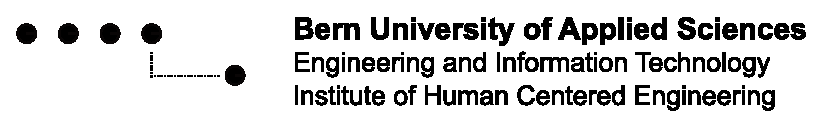
\includegraphics[height=0.5cm]{figs/BFHhuceENnofonts}}
\fancyhead[LO]{
\includegraphics[height=0.5cm]{figs/HuCEmicrolab-nofont}}
\fancyfoot[LE,RO]{\thepage}
\renewcommand{\headrulewidth}{0.4pt}
%-----------------------------------------------------------------------------
%
%%%%%%%%%%%%%%%%%%%%%%%%%%%%%%%%%%%%%%%%%%%%%%%%%%%%%%%%%%%%%%%%%%%%%%%%%%%%%%%%
%%            _   _            __   ____                                      %%
%%           / / | |          / _| |  __|                                     %%
%%           | |_| |  _   _  / /   | |_                                       %%
%%           |  _  | | | | | | |   |  _|                                      %%
%%           | | | | | |_| | \ \_  | |__                                      %%
%%           |_| |_| \_____|  \__| |____| microLab                            %%
%%                                                                            %%
%%           Bern University of Applied Sciences (BFH)                        %%
%%           Quellgasse 21                                                    %%
%%           Room HG 4.33                                                     %%
%%           2501 Biel/Bienne                                                 %%
%%           Switzerland                                                      %%
%%                                                                            %%
%%           http://www.microlab.ch                                           %%
%%%%%%%%%%%%%%%%%%%%%%%%%%%%%%%%%%%%%%%%%%%%%%%%%%%%%%%%%%%%%%%%%%%%%%%%%%%%%%%%
\chapter{Bus transactions}
\label{appen:bus}
This appendix describes the timing diagram of valid bus transactions and
transactions containing errors. Although the timing diagrams are shown for a
three datum burst transaction, it also reflects the single datum transaction.
%-----------------------------------------------------------------------------
\section{Write transactions}
In the write transaction the data flows from the user FPGA towards the {\sc
GECKO4com}. The timing diagram of a correct write transaction is shown in
Figure~\ref{fig:write correct}.
A write transaction is initiated by activating the $\overline{\textbf{start
trans}}$ signal and sending the \emph{Transmission Control Word (TCW)} (see
Chapter~\ref{sec:bus prot} and Figure~\ref{fig:TCW}) over the \textbf{data
cntrl} lines.\\
\textit{Important: All signals are active for one clock period of the
\textbf{bus clock}.\important}
\begin{figure}[hb]
\centering%
\includegraphics[width=\columnwidth]{figs/write_transaction_no_bus_error}
\caption{A correct write transaction that causes no bus error. Here a 3-short
burst transaction is shown. The blue lines represent tri-stated FPGA pins.}
\label{fig:write correct}
\end{figure}
 \\
After the initiation of the write transaction the user FPGA has to wait for the
{\sc GECKO4com} to activate the $\overline{\textbf{start send}}$ signal
(dependency \ding{'312}). Sending data before this dependency will result in
unpredictable results. After the reception of the $\overline{\textbf{start
send}}$ signal the user FPGA may start transmitting the data payload(shown by
\ding{'313}). The data payload may be a continues stream or chunk-ed into parts.
For each datum the user FPGA has to put the datum on the \textbf{data cntrl}
lines and activate both the $\overline{\textbf{valid lo}}$ and
$\overline{\textbf{valid hi}}$ lines to indicate valid data. After the sending
of the last datum, the user FPGA has to end the transaction by activating the
$\overline{\textbf{end trans}}$ signal as shown at \ding{'314}. The
$\overline{\textbf{end trans}}$ signal may be activated after or in parallel
with the sending of the last datum of the payload.\\
\textit{Important: the {\sc GECKO4com} does not check whether or not the user
FPGA sends the correct number of data. It assumes that the user FPGA does send
the number of data as announced in the Transmission Control Word (TCW).\important}
%-----------------------------------------------------------------------------
\section{Write transaction aborts}
Write transactions can be aborted under the conditions described in
Chapter~\ref{sec:mem map}. An aborted transaction is indicated by the {\sc
GECKO4com} by the activation of the $\overline{\textbf{error}}$ line. This
condition can occur anywhere during the transaction. Figure~\ref{fig:write
error 1} and Figure~\ref{fig:write error 2} show two examples of aborted write
transactions.
\begin{figure}[pt]
\centering%
\includegraphics[width=\columnwidth]{figs/write_transaction_bus_error_1}
\caption{An aborted write transaction before the reception of the
$\overline{\textbf{start trans}}$ signal.}
\label{fig:write error 1}
\end{figure}
\begin{figure}[pb]
\centering%
\includegraphics[width=\columnwidth]{figs/write_transaction_bus_error_2}
\caption{An aborted write transaction after the reception of the
$\overline{\textbf{start trans}}$ signal.}
\label{fig:write error 2}
\end{figure}
After the reception of the activated $\overline{\textbf{error}}$ signal the user
FPGA is required to activate the $\overline{\textbf{end trans}}$ signal to end
the transaction (as shown in dependency \ding{'315}).\\
\textit{Important: Failing to adhere to dependency \ding{'315} may leave the bus
in an undefined state.\important}
%-----------------------------------------------------------------------------
\section{Read transactions}
Simular to the write transaction a read transaction is initiated  by activating the $\overline{\textbf{start
trans}}$ signal and sending the \emph{Transmission Control Word (TCW)} (see
Chapter~\ref{sec:bus prot} and Figure~\ref{fig:TCW}) over the \textbf{data
cntrl} lines. As during the read transaction the data has to flow from the {\sc
GECKO4com} to the user FPGA the controlling of the bi-directional signals, shown
in  Table~\ref{tab:gecko4 bus signals}, need special attention.
Figure~\ref{fig:read correct} depicts a none-aborted read transaction for a
burst of three. 
\begin{figure}[t]
\centering%
\includegraphics[width=\columnwidth]{figs/read_transaction_no_bus_error}
\caption{A correct read transaction that causes no bus error. Here a 3-short
burst transaction is shown. The blue lines represent tri-stated FPGA pins.}
\label{fig:read correct}
\end{figure}
One cycle after the initialization of a read transaction (\ding{206}) the user
FPGA has to tristate all bi-directional signals. The user FPGA has to keep the
bi-directional signals in tristate up to one cycle after receiving an activated
$\overline{\textbf{end trans}}$ signal (\ding{208}).\\
\textit{Important: Failing to adhere to dependency \ding{206} and dependency \ding{208} may
destroy the IOB buffers of either or both the user FPGA and the {\sc GECKO4com}
FPGA!\important}\\
Two cycles after the reception of a read transaction (\ding{206}) the {\sc GECKO4com} will
start driving the bi-directional signals. The {\sc GECKO4com} will send the
requested number of shorts in one continues burst (\ding{207}) over the \textbf{data cntrl}
lines and activates the $\overline{\textbf{valid low}}$ and
$\overline{\textbf{valid low}}$ as described in Chapter~\ref{sec:bus prot}. During the transmission of the last datum of the read transaction
the {\sc GECKO4com} ends the transmission by activation of the
$\overline{\textbf{end trans}}$ signal. The \textbf{bus clock} cycle after the
activation of the $\overline{\textbf{end trans}}$ signal the {\sc GECKO4com}
puts all the bi-directional signals in three-state.\newpage
\textit{Important: The user FPGA has to make sure it has enough buffer capacity
to store the requested amount of data, as there is no way to interrupt the data
flow coming from the {\sc GECKO4com}.\important}
%-----------------------------------------------------------------------------
\section{Read transactions abort}
Read transactions can be aborted under the conditions described in
Chapter~\ref{sec:mem map}. An aborted transaction is indicated by the {\sc
GECKO4com} by the activation of the $\overline{\textbf{error}}$ line together
with the activation of the $\overline{\textbf{end trans}}$ signal (\ding{209}). 
Figure~\ref{fig:read error} shows an aborted read transaction.
\begin{figure}[t]
\centering%
\includegraphics[width=\columnwidth]{figs/read_transaction_bus_error}
\caption{An aborted read transaction. The blue lines represent tri-stated FPGA pins.}
\label{fig:read error}
\end{figure}

%
%-----------------------------------------------------------------------------
%
%%%%%%%%%%%%%%%%%%%%%%%%%%%%%%%%%%%%%%%%%%%%%%%%%%%%%%%%%%%%%%%%%%%%%%%%%%%%%%%%
%%            _   _            __   ____                                      %%
%%           / / | |          / _| |  __|                                     %%
%%           | |_| |  _   _  / /   | |_                                       %%
%%           |  _  | | | | | | |   |  _|                                      %%
%%           | | | | | |_| | \ \_  | |__                                      %%
%%           |_| |_| \_____|  \__| |____| microLab                            %%
%%                                                                            %%
%%           Bern University of Applied Sciences (BFH)                        %%
%%           Quellgasse 21                                                    %%
%%           Room HG 4.33                                                     %%
%%           2501 Biel/Bienne                                                 %%
%%           Switzerland                                                      %%
%%                                                                            %%
%%           http://www.microlab.ch                                           %%
%%%%%%%%%%%%%%%%%%%%%%%%%%%%%%%%%%%%%%%%%%%%%%%%%%%%%%%%%%%%%%%%%%%%%%%%%%%%%%%%
\chapter{{\sc GECKO4com} IO}
\label{appen:4com}
This appendix describes the different IO components and the connection diagrams.
\section{VGA screen and message windows}
Figure~\ref{fig:vga screenshot} show the VGA screen produced by the {\sc GECKO4com}. In
Figure~\ref{fig:vga screenshot} the three different text screens are marked in brown.
\begin{figure}[h]
\centering%
\includegraphics[width=\columnwidth]{figs/vga_screens}
\caption{The VGA screen as produced by the {\sc GECKO4com}. The different
message windows are marked in brown.}
\label{fig:vga screenshot}
\end{figure}
\section{Buttons, switch and LEDs}
Figure~\ref{fig:but sw leds} shows the {\sc GECKO4com}'s part of the {\sc GECKO4main}. The
different buttons, the switch and the bicolor LEDs are marked.
\begin{figure}[h]
\centering%
\includegraphics[width=\columnwidth]{figs/gecko4com}
\caption{The buttons, the switch and the LEDs of the {\sc GECKO4com}.}
\label{fig:but sw leds}
\end{figure}
\newpage
\section{VGA connection and RS232}
The bottom of Figure~\ref{fig:but sw leds} shows the {\sc GECKO4main}'s dual function connector and
its pin numbering.
This connector can be used to connect a VGA-screen and a
RS232 connector. Table~\ref{tab: conn vga rs232} lists the pin-numbers of this connector, the
corresponding signal names and their connection on a female VGA connector,
respectively their connections on a female RS232 connector. All signals not
listed in Table~\ref{tab: conn vga rs232} should be left unconnected.\\
\textit{Note: The 3.3V power supply can be used to supply level translators for
the RS232 communication (for example the MAX232).\note}
\begin{table}[h]
\centering%
\begin{tabular}{|c|l|c|}
\hline
\textbf{Dual function pin}&\textbf{Signal name}&\textbf{VGA pin}\\
\hline
\hline
\verb+1+&Ground&\verb+5,10+\\
\hline
\verb+3+&Vertical Sync&\verb+14+\\
\hline
\verb+4+&Horizontal Sync&\verb+13+\\
\hline
\verb+10+&Blue&\verb+3+\\
\hline
\verb+12+&Green&\verb+2+\\
\hline
\verb+13+&Analog Ground&\verb+6,7,8+\\
\hline
\verb+14+&Red&\verb+1+\\
\hline
\hline
\textbf{Dual function pin}&\textbf{Signal name}&\textbf{RS232 pin}\\
\hline
\hline
\verb+2+&\multicolumn{2}{c|}{3.3V power supply}\\
\hline
\verb+7+&RS232 RxD&\verb+3+\\
\hline
\verb+9+&RS232 TxD&\verb+2+\\
\hline
\verb+11+&Ground&\verb+5+\\
\hline
\end{tabular}
\caption{Connection diagram of the dual function connector to a VGA connector
and a RS232 connector (9-pol. Zero Modem connection)}
\label{tab: conn vga rs232}
\end{table}

%
%-----------------------------------------------------------------------------
%
\backmatter
%
%-----------------------------------------------------------------------------
%
\renewcommand{\headrulewidth}{0pt}
\fancyhead[LE,RO,LO,RE]{}
\fancyfoot[LE,RO]{\thepage}
\end{document}
